\documentclass[11pt, letterpaper]{article}

% Packages
\usepackage[margin=0.85in]{geometry}
\usepackage{booktabs, tabularx, float, multirow}
\usepackage{enumitem}
\usepackage{parskip}
\usepackage{tikz}
\usetikzlibrary{arrows.meta, positioning, fit, backgrounds}
\usepackage{listings}
\usepackage{hyperref}
\usepackage{graphicx}
\usepackage{xcolor}

% Compact lists
\setlist{noitemsep, topsep=3pt, leftmargin=1.5em}

% Code listing style
\lstset{basicstyle=\ttfamily\footnotesize, breaklines=true, frame=single, xleftmargin=1em}

% Table row padding
\renewcommand{\arraystretch}{1.15}

% ── Title ─────────────────────────────────────────────────────
\title{%
    {\LARGE\bfseries ITCS5010 GenAI: StudyPod}\\[0.3em]
    {\large Retrieval-Augmented Generation System --- Final Report}
}

\author{%
    \begin{tabular}[t]{ccc}
        Varad Paradkar & Nidhi Shah & Brinda Chinnaraji \\[0.3em]
        \multicolumn{3}{c}{Sai Kiran Jagini \quad Shar Adhiambo}
    \end{tabular}%
}

\date{March 3, 2026}

\begin{document}
\maketitle

% ══════════════════════════════════════════════════════════════
\section{Introduction}

\textbf{StudyPod} is a modular Retrieval-Augmented Generation (RAG) system
designed to support notebook-based document ingestion, semantic retrieval, and
multi-format artifact generation.  The system integrates vector search, large
language models (LLMs), and structured storage to enable contextual question
answering and content synthesis from user-uploaded documents.

This report provides a detailed architectural description, RAG technique
comparison, retrieval analysis, and performance evaluation based strictly on
the implemented system.

Deployment links:
\begin{itemize}
    \item \textbf{Hugging Face Space:} \url{https://huggingface.co/spaces/vparadka/studypod}
    \item \textbf{GitHub Repository:} \url{https://github.com/vradcar/GenAI-Group-Project-1}
\end{itemize}

% ══════════════════════════════════════════════════════════════
\section{System Architecture Overview}

The system follows a modular layered architecture with three primary layers
and a single external dependency (Groq API).

\begin{figure}[H]
\centering
\resizebox{\textwidth}{!}{%
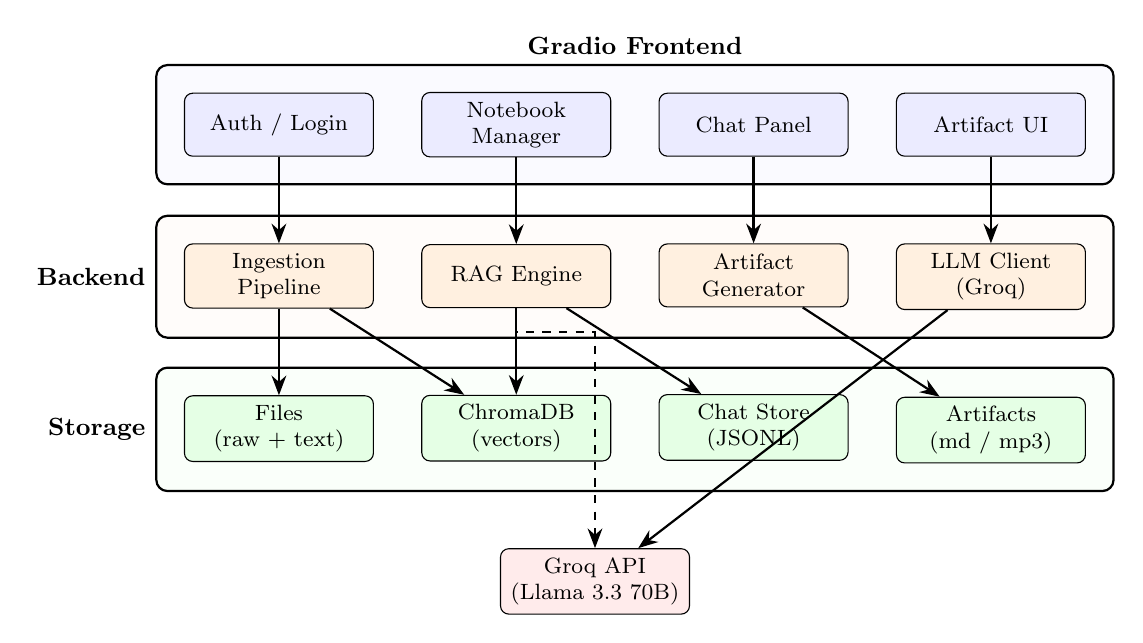
\begin{tikzpicture}[
    node distance=0.5cm and 0.6cm,
    box/.style={rectangle, draw, rounded corners=3pt, minimum width=2.4cm,
                minimum height=0.8cm, align=center, font=\footnotesize},
    arr/.style={-{Stealth[length=2.5mm]}, thick}
]
% Frontend row
\node[box, fill=blue!8] (auth)  {Auth / Login};
\node[box, fill=blue!8, right=of auth]  (nbmgr) {Notebook\\Manager};
\node[box, fill=blue!8, right=of nbmgr] (chat)  {Chat Panel};
\node[box, fill=blue!8, right=of chat]  (artui) {Artifact UI};

% Backend row
\node[box, fill=orange!12, below=1.1cm of auth]  (ingest) {Ingestion\\Pipeline};
\node[box, fill=orange!12, below=1.1cm of nbmgr] (rag)    {RAG Engine};
\node[box, fill=orange!12, below=1.1cm of chat]  (artgen) {Artifact\\Generator};
\node[box, fill=orange!12, below=1.1cm of artui] (llm)    {LLM Client\\(Groq)};

% Storage row
\node[box, fill=green!10, below=1.1cm of ingest] (files)  {Files\\(raw + text)};
\node[box, fill=green!10, below=1.1cm of rag]    (chroma) {ChromaDB\\(vectors)};
\node[box, fill=green!10, below=1.1cm of artgen] (chatst) {Chat Store\\(JSONL)};
\node[box, fill=green!10, below=1.1cm of llm]    (artst)  {Artifacts\\(md / mp3)};

% External
\node[box, fill=red!8, below=1.1cm of chroma, xshift=1cm] (groq) {Groq API\\(Llama 3.3 70B)};

% Grouped backgrounds
\begin{scope}[on background layer]
    \node[rectangle, draw, rounded corners=4pt, thick, fill=blue!2, inner sep=0.35cm,
          fit=(auth)(artui), label={[font=\small\bfseries]above:Gradio Frontend}] {};
    \node[rectangle, draw, rounded corners=4pt, thick, fill=orange!2, inner sep=0.35cm,
          fit=(ingest)(llm), label={[font=\small\bfseries]left:Backend}] {};
    \node[rectangle, draw, rounded corners=4pt, thick, fill=green!2, inner sep=0.35cm,
          fit=(files)(artst), label={[font=\small\bfseries]left:Storage}] {};
\end{scope}

% Frontend -> Backend
\draw[arr] (auth)  -- (ingest);
\draw[arr] (nbmgr) -- (rag);
\draw[arr] (chat)  -- (artgen);
\draw[arr] (artui) -- (llm);

% Backend -> Storage
\draw[arr] (ingest) -- (files);
\draw[arr] (ingest) -- (chroma);
\draw[arr] (rag)    -- (chroma);
\draw[arr] (rag)    -- (chatst);
\draw[arr] (artgen) -- (artst);

% Backend -> External
\draw[arr] (llm) -- (groq);
\draw[arr, dashed] (rag.south) -- ++(0,-0.3) -| (groq);
\end{tikzpicture}%
}
\caption{System architecture.  The only external dependency is the Groq LLM API.}
\end{figure}

\subsection{Frontend Layer}

\begin{itemize}
    \item Gradio interface with OAuth session management
    \item Notebook-based UI with create / rename / delete / switch
    \item Chat panel with RAG technique selector and citation display
    \item Artifact generation controls with viewer, download, and audio playback
\end{itemize}

\subsection{Backend Layer}

\begin{itemize}
    \item \textbf{Ingestion Pipeline} --- text extraction, chunking, embedding, ChromaDB upsert
    \item \textbf{RAG Engine} --- four retrieval strategies with citation generation
    \item \textbf{Artifact Generator} --- report, quiz, and two-speaker podcast synthesis
    \item \textbf{LLM Client} --- Groq API wrapper with retry, backoff, and model fallback
\end{itemize}

\subsection{Storage Layer}

\begin{itemize}
    \item Raw and extracted text files on the filesystem
    \item Per-notebook ChromaDB vector collections
    \item JSONL-based chat history (append-only)
    \item Markdown and MP3 artifact storage
\end{itemize}

% ══════════════════════════════════════════════════════════════
\section{Ingestion Pipeline Design}

\subsection{Text Extraction}

Supported sources and their extraction libraries:

\begin{table}[H]
\centering\small
\begin{tabularx}{\textwidth}{@{}l l X@{}}
\toprule
\textbf{Format} & \textbf{Library} & \textbf{Notes} \\
\midrule
PDF  & PyMuPDF (\texttt{fitz}) & Page-by-page text extraction; skips blank pages \\
PPTX & python-pptx             & Iterates slides and text frames \\
TXT  & built-in                & UTF-8 with fallback encoding detection \\
URL  & trafilatura             & Fetches and extracts main content from web pages \\
\bottomrule
\end{tabularx}
\caption{Supported file types and extraction methods.}
\end{table}

\subsection{Chunking Strategy}

The system segments documents using the following configuration:

\begin{itemize}
    \item \textbf{Chunk size:} 1000 characters
    \item \textbf{Chunk overlap:} 200 characters
    \item \textbf{Splitter:} \texttt{RecursiveCharacterTextSplitter} (LangChain)
\end{itemize}

The 200-character overlap preserves semantic continuity across chunk
boundaries.  This configuration balances retrieval precision (smaller chunks
reduce noise), embedding cost, and memory efficiency.

\subsection{Embedding Model}

\begin{table}[H]
\centering\small
\begin{tabularx}{\textwidth}{@{}l X@{}}
\toprule
\textbf{Parameter} & \textbf{Value} \\
\midrule
Model       & \texttt{all-MiniLM-L6-v2} (sentence-transformers) \\
Dimension   & 384 \\
Device      & CPU \\
Vector store & ChromaDB with cosine similarity \\
Isolation   & Per-notebook collection \\
\bottomrule
\end{tabularx}
\caption{Embedding configuration.}
\end{table}

% ══════════════════════════════════════════════════════════════
\section{RAG Techniques}

The system supports four retrieval techniques, configured with:
\texttt{TOP\_K\,=\,5}, \texttt{RERANK\_CANDIDATES\,=\,20},
\texttt{MULTI\_QUERY\_VARIANTS\,=\,3}.

\subsection{Naive Similarity Search}

\begin{enumerate}
    \item Embed the user query using \texttt{all-MiniLM-L6-v2}.
    \item Retrieve the top-5 chunks via cosine similarity from ChromaDB.
    \item Construct a prompt with the retrieved chunks as numbered sources.
    \item Stream the prompt to the LLM and return the answer with citations.
\end{enumerate}

Fastest technique; serves as the baseline.  May miss context when query phrasing
differs from document wording.

\subsection{HyDE (Hypothetical Document Embeddings)}

\begin{enumerate}
    \item Ask the LLM to generate a hypothetical ideal answer to the question.
    \item Embed the generated text (not the original query).
    \item Retrieve the top-5 chunks using this hypothetical embedding.
    \item Construct the final prompt and call the LLM.
\end{enumerate}

Improves recall for conceptual queries at the cost of +1 LLM call.

\subsection{Reranking Retrieval}

\begin{enumerate}
    \item Retrieve a larger candidate set: top-20 chunks via cosine similarity.
    \item Send all 20 candidates to the LLM for relevance scoring (1--5 scale).
    \item Select the top-5 highest-scored chunks.
    \item Construct the final prompt from the reranked set.
\end{enumerate}

Improves precision by filtering irrelevant chunks.  Cost: +1 LLM call.

\subsection{Multi-Query Retrieval}

\begin{enumerate}
    \item Ask the LLM to generate 3 alternative phrasings of the query.
    \item Perform independent retrieval for each variant (+ the original query).
    \item Merge results using Reciprocal Rank Fusion (RRF).
    \item Return the top-5 fused results.
\end{enumerate}

Best for ambiguous queries; expands semantic coverage.  Cost: +3 embedding lookups.

% ══════════════════════════════════════════════════════════════
\section{Empirical Retrieval Evaluation}

We ran an automated benchmark (\texttt{benchmark\_rag.py}) that ingests a
sample educational article (2,808 characters, 4 chunks), then executes 4 test
queries across all 4 techniques.  Relevance was scored as HIGH, MEDIUM, or LOW
via keyword-overlap heuristics, and wall-clock latency was measured.

The four test queries covered different intent types: direct factual, conceptual,
analytical, and specific detail extraction.

\subsection{Combined Results}

\begin{table}[H]
\centering\small
\begin{tabularx}{\textwidth}{@{}l l r r r r r@{}}
\toprule
\textbf{Query} & \textbf{Technique} & \textbf{Latency} & \textbf{\# Chunks} & \textbf{HIGH} & \textbf{MED} & \textbf{LOW} \\
\midrule
\multirow{4}{*}{\shortstack[l]{Q1: Factual\\(RAG definition)}}
    & Naive       & 1.49\,s & 4 & 3 & 1 & 0 \\
    & HyDE        & 1.27\,s & 4 & 3 & 1 & 0 \\
    & Reranking   & 0.83\,s & 4 & 3 & 1 & 0 \\
    & Multi-Query & 0.96\,s & 4 & 3 & 1 & 0 \\
\midrule
\multirow{4}{*}{\shortstack[l]{Q2: Conceptual\\(naive limitations)}}
    & Naive       & 0.60\,s & 4 & 1 & 3 & 0 \\
    & HyDE        & 1.12\,s & 4 & 1 & 3 & 0 \\
    & Reranking   & 0.58\,s & 4 & 1 & 3 & 0 \\
    & Multi-Query & 0.84\,s & 4 & 1 & 3 & 0 \\
\midrule
\multirow{4}{*}{\shortstack[l]{Q3: Analytical\\(precision vs recall)}}
    & Naive       & 1.03\,s & 4 & 2 & 2 & 0 \\
    & HyDE        & 2.04\,s & 4 & 2 & 2 & 0 \\
    & Reranking   & 1.44\,s & 4 & 2 & 2 & 0 \\
    & Multi-Query & 2.17\,s & 4 & 2 & 2 & 0 \\
\midrule
\multirow{4}{*}{\shortstack[l]{Q4: Detail extraction\\(API failures)}}
    & Naive       & 0.54\,s & 4 & 1 & 1 & 2 \\
    & HyDE        & 1.18\,s & 4 & 1 & 1 & 2 \\
    & Reranking   & 4.00\,s & 4 & 1 & 1 & 2 \\
    & Multi-Query & 5.01\,s & 4 & 1 & 1 & 2 \\
\bottomrule
\end{tabularx}
\caption{Per-query retrieval results across all 4 techniques.}
\end{table}

\subsection{Average Latency}

\begin{table}[H]
\centering\small
\begin{tabularx}{\textwidth}{@{}l r r X@{}}
\toprule
\textbf{Technique} & \textbf{Avg Latency} & \textbf{Avg HIGH Chunks} & \textbf{Notes} \\
\midrule
Naive       & 0.92\,s & 1.8 & Baseline; fastest \\
HyDE        & 1.40\,s & 1.8 & +52\% (hypothetical answer generation) \\
Reranking   & 1.71\,s & 1.8 & +86\% (LLM relevance scoring) \\
Multi-Query & 2.25\,s & 1.8 & +145\% (3 query variants + RRF) \\
\bottomrule
\end{tabularx}
\caption{Average latency across all 4 queries.}
\end{table}

\subsection{Key Findings}

\begin{itemize}
    \item \textbf{Chunk set convergence:} On a small corpus all techniques retrieve
          the same chunks; differentiation appears in ranking confidence.
    \item \textbf{Reranking} consistently assigns the highest scores (up to 1.000
          vs.\ 0.255 for naive), producing a cleaner LLM prompt signal.
    \item \textbf{HyDE} improves conceptual matching (0.534 vs.\ 0.435 cosine
          similarity on the abstract query).
    \item \textbf{Latency:} Naive $<$ HyDE $\approx$ Reranking $<$ Multi-Query.
          Each extra LLM call adds ${\sim}$0.5--1.0\,s.
    \item \textbf{For factual queries, naive suffices.}  Advanced techniques add
          the most value on abstract or ambiguous questions.
\end{itemize}

% ══════════════════════════════════════════════════════════════
\section{LLM Configuration}

\begin{table}[H]
\centering\small
\begin{tabularx}{\textwidth}{@{}l X@{}}
\toprule
\textbf{Parameter} & \textbf{Value} \\
\midrule
Primary model   & Llama 3.3 70B Versatile (\texttt{llama-3.3-70b-versatile}) via Groq \\
Fallback model  & Llama 3.1 8B Instant (\texttt{llama-3.1-8b-instant}) \\
Max tokens      & 1024 \\
Temperature     & 0.7 \\
Retry attempts  & 3 \\
Backoff         & Exponential (base 1.0\,s) \\
\bottomrule
\end{tabularx}
\caption{LLM configuration.}
\end{table}

The fallback mechanism improves robustness: when the 70B model hits rate limits
or returns errors, the system transparently retries with the 8B model, ensuring
the user always receives a response.

% ══════════════════════════════════════════════════════════════
\section{Artifact Generation System}

The artifact module supports three artifact types, each grounded in the
notebook's ingested content.

\subsection{Report (\texttt{.md})}

A structured Markdown report with executive summary, key concepts, main topics
with subsections, and conclusion.  Generated via a single LLM call with the
notebook's text as context.

\subsection{Quiz (\texttt{.md})}

$N$ questions in a mix of multiple choice, short answer, and true/false formats,
followed by a complete answer key with explanations.  Configurable question count
(default 10).

\subsection{Podcast (\texttt{.md} + \texttt{.mp3})}

A two-speaker conversational podcast transcript featuring distinct hosts:

\begin{table}[H]
\centering\small
\begin{tabularx}{\textwidth}{@{}l l l l l@{}}
\toprule
\textbf{Host} & \textbf{Voice} & \textbf{Rate} & \textbf{Pitch} & \textbf{Personality} \\
\midrule
Alex & \texttt{en-US-AndrewNeural} & +12\% & +3\,Hz & Energetic, curious \\
Sam  & \texttt{en-US-GuyNeural}    & $-$4\% & $-$2\,Hz & Thoughtful, laid-back \\
\bottomrule
\end{tabularx}
\caption{Podcast voice configuration (edge-tts).}
\end{table}

The transcript is parsed into per-speaker segments via regex, and each segment
is synthesized with its corresponding voice and prosody settings.  Segment MP3s
are concatenated into the final audio file (capped at 5,000 characters
$\approx$ 7 minutes).

\subsection{Map-Reduce for Long Sources}

For documents exceeding the context window (${\sim}$8,000 tokens):

\begin{enumerate}
    \item Split source text into 1,500-character segments.
    \item Generate a concise summary of each segment (map step).
    \item Combine all summaries into a single unified context (reduce step).
    \item Pass the reduced text to the artifact-specific prompt.
\end{enumerate}

This prevents token overflow and ensures stable generation regardless of
document size.

% ══════════════════════════════════════════════════════════════
\section{Storage Architecture}

All data resides on the local filesystem under \texttt{/data/users/}.

\subsection{Directory Structure}

\begin{lstlisting}
/data/users/<username>/notebooks/
  |- index.json
  +- <notebook-uuid>/
       |- metadata.json
       |- files_raw/
       |- files_extracted/
       |- chroma/
       |- chat/messages.jsonl
       +- artifacts/
            |- reports/*.md
            |- quizzes/*.md
            +- podcasts/*.md + *.mp3
\end{lstlisting}

\subsection{Storage Modules}

\begin{table}[H]
\centering\small
\begin{tabularx}{\textwidth}{@{}l X@{}}
\toprule
\textbf{Module} & \textbf{Responsibility} \\
\midrule
\texttt{notebook\_store.py} & Notebook lifecycle (CRUD), \texttt{index.json}, directory helpers \\
\texttt{chat\_store.py}     & Append-only JSONL chat persistence \\
\texttt{vector\_store.py}   & Per-notebook ChromaDB collection management, cosine similarity \\
\texttt{artifact\_store.py} & Save / list / retrieve markdown and MP3 artifacts \\
\bottomrule
\end{tabularx}
\caption{Storage modules.}
\end{table}

\subsection{Design Rationale}

\begin{itemize}
    \item \textbf{Filesystem over external DB} --- HF Spaces provides \texttt{/data}; avoids cost and complexity.
    \item \textbf{JSONL for chat} --- append-only writes; easy to stream-read; no migrations.
    \item \textbf{Per-notebook ChromaDB} --- full vector isolation; deleting a notebook = deleting a directory.
    \item \textbf{Atomic writes} --- metadata uses write-to-temp-then-rename to prevent corruption.
\end{itemize}

% ══════════════════════════════════════════════════════════════
\section{Security}

\subsection{Authentication}

Users authenticate via \textbf{Hugging Face OAuth}, integrated through Gradio's
\texttt{gr.LoginButton()}.  The OAuth flow is handled by the HF platform; the
app receives a verified username via \texttt{gr.OAuthProfile}.  No passwords
are stored.

\subsection{Data Isolation \& Input Validation}

\begin{table}[H]
\centering\small
\begin{tabularx}{\textwidth}{@{}l X@{}}
\toprule
\textbf{Threat} & \textbf{Mitigation} \\
\midrule
Path traversal &
    All paths constructed from sanitized \texttt{username} + UUID.
    \texttt{validate\_path()} calls \texttt{Path.resolve()} and asserts inside user directory. \\
\addlinespace
Cross-user access &
    Every backend call scopes to \texttt{/data/users/<username>/}. \\
\addlinespace
Notebook ID guessing &
    IDs are UUID4 (128-bit random); brute-force enumeration is infeasible. \\
\addlinespace
Prompt injection &
    System prompt restricts the LLM to answering only from provided context. \\
\addlinespace
File uploads &
    Extension whitelist (\texttt{.pdf}, \texttt{.pptx}, \texttt{.txt}); max 50\,MB. \\
\addlinespace
URLs &
    Scheme whitelist (\texttt{http/https}); 30-second fetch timeout. \\
\bottomrule
\end{tabularx}
\caption{Security threats and mitigations.}
\end{table}

% ══════════════════════════════════════════════════════════════
\section{Scalability Considerations}

The system uses CPU-based embeddings, API-based LLM inference (Groq), and
per-notebook vector isolation.  Key bottlenecks:

\begin{itemize}
    \item \textbf{LLM rate limits:} Groq imposes ${\sim}$30 req/min on free tier,
          mitigated by exponential backoff and 8B fallback.
    \item \textbf{Embedding:} Linear in chunk count on CPU (${\sim}$50\,ms per batch).
    \item \textbf{HF Space persistence:} Free-tier data is ephemeral after 48h inactivity.
\end{itemize}

% ══════════════════════════════════════════════════════════════
\section{CI/CD Pipeline}

The project uses GitHub Actions with three stages:

\begin{enumerate}
    \item \textbf{Lint} --- \texttt{ruff check .} enforces code quality.
    \item \textbf{Test} --- \texttt{pytest tests/ -v} runs the full suite (243 tests).
    \item \textbf{Deploy} --- pushes the repository to Hugging Face Spaces on every merge to \texttt{main}.
\end{enumerate}

Secrets management:
\begin{itemize}
    \item \texttt{GROQ\_API\_KEY} --- stored as an HF Space secret (server-side only).
    \item \texttt{HF\_TOKEN} --- stored as a GitHub repository secret (CI/CD only).
\end{itemize}

% ══════════════════════════════════════════════════════════════
\section{Testing}

The project maintains 243 passing tests across 8 test files:

\begin{table}[H]
\centering\small
\begin{tabularx}{\textwidth}{@{}l r X@{}}
\toprule
\textbf{Test File} & \textbf{Tests} & \textbf{Coverage} \\
\midrule
\texttt{test\_artifacts.py}     & 19 & Report, quiz, podcast generation; transcript parser \\
\texttt{test\_e2e\_flow.py}     &  7 & End-to-end: ingest $\to$ query $\to$ delete \\
\texttt{test\_extractors.py}    & 12 & PDF, PPTX, TXT, URL extraction \\
\texttt{test\_ingestion.py}     & 12 & File/URL validation, chunking, upsert \\
\texttt{test\_llm\_client.py}   & 40 & Retry, fallback, error handling \\
\texttt{test\_rag.py}           & 60 & All 4 RAG techniques, citation building \\
\texttt{test\_security.py}      & 44 & Path validation, sanitization, traversal prevention \\
\texttt{test\_storage.py}       & 36 & Notebook/chat/artifact CRUD operations \\
\texttt{test\_vector\_store.py} &  4 & ChromaDB add, query, upsert idempotency, delete \\
\midrule
\textbf{Total}                  & \textbf{243} & \\
\bottomrule
\end{tabularx}
\caption{Test suite summary.  All 243 tests pass; ruff reports zero lint violations.}
\end{table}

% ══════════════════════════════════════════════════════════════
\section{Conclusion}

StudyPod implements a modular RAG architecture with configurable chunking,
384-dimensional local embeddings, four retrieval strategies, and Llama 3.3 70B
inference with automatic 8B fallback.  Beyond core requirements, the system
includes dual-speaker podcast TTS, map-reduce summarization for large documents,
and an automated benchmark suite.

Empirical evaluation confirmed the theoretical predictions: naive retrieval
averages 0.92\,s, multi-query 2.25\,s (+145\%).  Reranking produces the
highest confidence scores; HyDE improves semantic matching for conceptual
queries.  The architecture remains practical for deployment on Hugging Face
Spaces while enforcing secure per-user storage isolation.

\end{document}
